\documentclass[11pt]{tg_usta}
% Informe PARCIAL 2 - NLP
% Plantilla basada en tg_usta.cls del TALLER-2 (PUJ)
\usepackage{tcolorbox}
\usepackage{float}
\usepackage{graphicx}
\usepackage{makecell}
\usepackage{anysize}
\usepackage{cite}
\marginsize{1in}{1in}{1in}{1in} %% Márgenes NO MODIFICAR
\usepackage{amsmath,amsthm,amssymb}
\usepackage{multicol}
\usepackage{url}
\usepackage{multirow}
\usepackage{array}
\usepackage{booktabs}
\usepackage[T1]{fontenc}
\usepackage[utf8]{inputenc}
\usepackage{subcaption}

\newtheorem{definicion}{Definición}[section]
\newtheorem{nota}{Nota}[section]
\allowdisplaybreaks
\decimalpoint

\begin{document}
\title[maintitle = Transferencia de conocimiento biomédico entre lenguas: análisis crítico de la destilación con Sentence Transformers,
       shorttitle = Destilación multilingüe y conocimiento biomédico,
       secondtitle = Parcial 2 - Procesamiento de Lenguaje Natural]

\begin{authors}[Rivera, Carrillo, Garnica \& Prieto]

\author[affiliation = PUJ,
        firstname = Erika Valeria,
        surname = Rivera Jimenez,
        email = riveraev@javeriana.edu.co]

\author[affiliation = PUJ,
        firstname = Julian Guillermo,
        surname = Carrillo Meneses,
        email = carrillojuliang@javeriana.edu.co]

\author[affiliation = PUJ,
        firstname = Carlos Andres,
        surname = Garnica Salazar,
        email = carlos\_garnicas@javeriana.edu.co]

\author[affiliation = PUJ,
        firstname = Oscar Andres,
        surname = Prieto Moreno,
        email = o-prieto@javeriana.edu.co]

\end{authors}

\begin{mainabstract}

Este informe analiza el artículo de Piperno et al. (2025) sobre destilación de conocimiento multilingüe con Sentence Transformers para clasificación temática en el dominio biomédico. El estudio traduce textos ingleses con mBART, alinea las representaciones de un profesor BioBERT o mBERT con un estudiante mBERT mediante Multiple Negatives Ranking Loss y ajusta el estudiante con etiquetas en español, francés y alemán. El máximo reportado es de 12,89 puntos de F1 con el 10\,\% de los datos; el promedio cae de 7,95 a 0,45 puntos al pasar del 10 al 100\,\%. El informe reconstruye el diseño, verifica las cifras, discute los límites de validez y responde dos preguntas del foro (cuándo justifica la destilación y qué evidencia exigiría su transferencia a Colombia) y tres de clase (transferencia de sesgos, mitigación y equivalencia semántica). La conclusión principal es que la destilación es una técnica de eficiencia de datos, no una garantía de equidad ni de validez clínica, y que su transferencia a textos médicos colombianos exige validación externa, anotación clínica y análisis de equidad. \\\\
\textit{\textbf{Palabras clave:}} Destilación de conocimiento, Sentence Transformers, modelos multilingües, dominio biomédico, sesgo, evaluación crítica

\end{mainabstract}

\section{Introducción}
\label{sec:introduccion}

El artículo \emph{Cross-lingual distillation for domain knowledge transfer with sentence transformers}, de Piperno, Bacco, Dell'Orletta, Merone y Pecchia, publicado en 2025 en el volumen 311 de \emph{Knowledge-Based Systems}, aborda la subrepresentación de las lenguas distintas del inglés en el procesamiento de lenguaje natural y elige el dominio biomédico \cite{piperno2025}. Su propuesta traduce textos médicos ingleses al español, al francés y al alemán con mBART, alinea las representaciones de un profesor entrenado en inglés con las de un estudiante mBERT mediante \emph{Multiple Negatives Ranking Loss} y ajusta el estudiante con etiquetas en la lengua destino usando entre el 10 y el 100\,\% de los datos. El máximo reportado es de 12,89 puntos de F1 con el 10\,\%; el promedio cae de 7,95 a 0,45 puntos al pasar al 100\,\%.

El trabajo se inscribe en el seminario «Más allá del modelo», cuyas pautas piden contar el artículo como una historia y separar lo que reportan los autores de la valoración del equipo \cite{moreno2026}. La lectura sigue esa indicación: no resume sección por sección, reconstruye el argumento y lo examina en los puntos donde la evidencia no alcanza.

Nuestra tesis es que la destilación es una técnica de eficiencia de datos, no una garantía de equidad ni de validez clínica. El artículo abre con un marco de inclusión tecnológica y cierra con la promesa de hacer accesible la información biomédica en varias lenguas, pero su diseño mide una sola cosa: la exactitud de un clasificador temático en tres lenguas europeas. Tres observaciones sostienen la tesis. La ganancia se concentra en el régimen de pocos datos y se desvanece cuando hay anotación suficiente. El término \emph{unbiased dataset} se refiere a la ausencia de solapamiento léxico entre el entrenamiento traducido y la prueba, no a sesgo social. La evaluación se hace sobre manuales médicos, no sobre texto clínico real, así que la validez externa hacia registros hospitalarios o hacia el español de Colombia queda sin comprobar.


\section{Problema y contexto}
\label{sec:problema}

El artículo parte de una observación conocida: los corpus anotados, las herramientas y los modelos preentrenados se concentran en inglés, y esa concentración reduce la calidad de los sistemas en otras lenguas \cite{piperno2025}. La consecuencia excede lo técnico. En principio, si un modelo no procesa bien el español médico, una institución queda atada a recursos en inglés o a servicios externos, y los hablantes reciben sistemas menos precisos para decisiones que afectan su salud \cite{piperno2025}.

\subsection{Las dos brechas}

mBERT ilustra la brecha lingüística: comparte un vocabulario de subpalabras entre 104 lenguas y se entrena con las Wikipedias más grandes \cite{devlin2019}. La cobertura no implica exposición equilibrada: el tamaño de las Wikipedias varía y los registros enciclopédicos no son los de una historia clínica. El modelo puede reconocer la lengua y carecer del vocabulario técnico que la tarea exige.

BioBERT ilustra la brecha de dominio: continúa el preentrenamiento de BERT sobre PubMed y PMC y mejora en varias tareas biomédicas, pero su conocimiento está en inglés \cite{lee2020}. mBERT es multilingüe, pero generalista. Cubrir ambas dimensiones con los medios habituales exige construir un modelo de dominio por lengua, con corpus anotado por especialistas. El costo de esa ruta es el argumento económico del artículo: la anotación clínica requiere especialistas, confidencialidad y tiempo, y se multiplica por cada lengua.

El vocabulario agrava el problema. Los términos médicos son largos, composicionales y poco frecuentes, y la tokenización por subpalabras los fragmenta \cite{lee2020}. El corpus separa material para profesionales y para pacientes: el mismo tema se escribe de maneras distintas según el destinatario, y el clasificador debe cubrir ambas.

\subsection{Alcance y pregunta central}

El español es una de las lenguas con más hablantes y cuenta con modelos generales propios, BETO y MarIA, que reducen la brecha lingüística pero no la de dominio \cite{canete2020,gutierrez2022}. La solución del artículo, importar el conocimiento inglés y alinearlo con un estudiante multilingüe, evita entrenar un modelo biomédico en español desde cero. Para América Latina, donde los recursos anotados en salud son escasos, ese ahorro tiene interés práctico.

Conviene precisar el alcance. El artículo no estudia variedades regionales. El corpus de destino combina manuales originales en cada lengua con traducciones automáticas del inglés para la destilación, y la evaluación se hace sobre textos originales de manuales, filtrados por su similitud con el entrenamiento traducido. No hay textos colombianos, mexicanos ni argentinos, ni términos locales, ni variación dialectal. El experimento responde una pregunta sobre transferencia entre lenguas, no sobre adecuación al español de una región.

La pregunta central es si es posible transferir conocimiento de dominio y de tarea desde un modelo entrenado en inglés hacia un estudiante multilingüe, usando pares traducidos y sin etiquetas inglesas en el ajuste final, y cómo cambia esa transferencia según la cantidad de anotación disponible. El diseño busca separar el conocimiento de dominio, que proviene del preentrenamiento, del conocimiento de tarea, que proviene del ajuste supervisado. Nuestra objeción no es a la pregunta sino a la respuesta: el artículo la contesta con promedios de F1 sobre tres lenguas y sin medidas de dispersión, de modo que el resultado dice qué ocurrió en esos experimentos, no cuánto puede esperarse en otro corpus.

\section{Antecedentes y aporte}
\label{sec:antecedentes}

El artículo ordena su campo en dos familias: alineación de vocabulario y destilación de conocimiento \cite{piperno2025}. La primera acerca las lenguas en el espacio de representaciones; la segunda transfiere el comportamiento de un modelo a otro. Piperno et al.\ pertenecen a la segunda, aunque usan traducción automática para construir los pares.

\subsection{Dos familias y un antecedente}

Los trabajos de alineación buscan que palabras equivalentes en dos lenguas ocupen posiciones cercanas en un espacio compartido. Se apoyan en diccionarios bilingües, corpus paralelos o señales no supervisadas. Su límite aparece cuando la tarea depende de estructura y contexto: alinear palabras no transfiere la conducta de un clasificador ni el conocimiento de las capas de un modelo preentrenado. El límite se agrava cuando no hay corpus paralelo ni diccionario bilingüe que sirva de señal.

Sentence-BERT es la infraestructura que hace medible la alineación: ajusta una red siamesa sobre BERT para que dos oraciones produzcan vectores comparables con similitud coseno \cite{reimers2019}. El antecedente directo es Reimers y Gurevych \cite{reimers2020}: un profesor monolingüe en inglés produce vectores, un estudiante multilingüe produce vectores para las oraciones y sus traducciones, y una pérdida de error cuadrático medio acerca ambos espacios. Piperno et al.\ adoptan ese esquema y lo declaran: su comparación principal es una reimplementación con MSE frente a su variante con MNRL. Lo que cambia es la pérdida, el dominio y el diseño experimental.

BERT aporta la arquitectura: un codificador bidireccional preentrenado con enmascaramiento de tokens y predicción de la oración siguiente \cite{devlin2019}. BioBERT continúa ese preentrenamiento con literatura biomédica \cite{lee2020}; mBERT repite la arquitectura y los objetivos sobre 104 lenguas con un vocabulario compartido; mBART es un modelo secuencia a secuencia preentrenado con denoising multilingüe \cite{liu2020}. En el artículo, mBART no se estudia: es la herramienta que produce las traducciones. Esa distinción importa porque la calidad de mBART fija el techo de la alineación y el artículo no la mide con métricas semánticas.

\subsection{Qué toma y qué aporta}

El artículo toma cuatro elementos: el marco de destilación a nivel de características, la asimetría profesor monolingüe y estudiante multilingüe con la traducción como puente, la infraestructura de Sentence Transformers y la pérdida MSE como referencia. Los autores son explícitos en que no proponen un método nuevo ni modifican los fundamentos de la destilación. El aporte es empírico.

El primer aporte es el uso de MNRL en este escenario. La pérdida no es una invención: los autores la presentan como novedad, pero no aportan una comparación que descarte usos previos de MNRL con pares traducidos. Su argumento es que tolera mejor el ruido que MSE; los resultados lo respaldan en 32 de 36 celdas. El segundo aporte es el diseño de profesores: BioBERT preentrenado, BioBERT ajustado y mBERT ajustado permiten contrastar el valor del dominio con el de la tarea.

El tercer aporte es el barrido de 10, 25, 50 y 100\,\% de datos, que muestra que el beneficio se concentra en pocos datos. El cuarto aporte es el RSA y la distancia entre matrices de confusión, que buscan evidencia de mecanismo y no solo de exactitud.

Nuestra valoración es que el aporte está en el diseño experimental y en la delimitación del escenario, no en la pérdida ni en la arquitectura. El artículo no compara su método con la alineación de vocabulario ni con el entrenamiento sobre traducciones, y tampoco incluye un codificador monolingüe en español como alternativa. Esa ausencia deja abierta la pregunta que más interesa a un lector latinoamericano: si el resultado se repetiría con BETO o MarIA.

\section{Preguntas y diseño experimental}
\label{sec:preguntas}

El artículo organiza su indagación en cinco preguntas que cubren la transferencia de dominio, la transferencia de tarea, el valor del preentrenamiento especializado, el efecto del tamaño de los datos y el cambio en las representaciones internas \cite{piperno2025}.

\begin{itemize}
  \item \textbf{Pregunta 1.} ¿Puede transferirse el conocimiento de dominio de un modelo preentrenado en ese dominio cuando no se dispone de datos etiquetados en inglés para la tarea?
  \item \textbf{Pregunta 2.} ¿Puede transferirse el conocimiento de tarea desde un modelo ajustado en inglés cuando ese tipo de datos sí existe?
  \item \textbf{Pregunta 3.} Si no hay un modelo adaptado al dominio disponible en inglés, ¿qué beneficios tiene destilar el conocimiento de tarea desde un modelo ajustado a partir del mismo punto de partida que el estudiante?
  \item \textbf{Pregunta 4.} ¿Cómo influye la cantidad de datos usada en el ajuste sobre el desempeño final?
  \item \textbf{Pregunta 5.} ¿Qué diferencias aparecen en las representaciones internas del profesor y del estudiante después de la destilación?
\end{itemize}

Las tres primeras se responden contrastando un profesor con otro. La pregunta 4 es de escala y se responde con la curva de desempeño. La pregunta 5 es de mecanismo y se responde con análisis de representaciones.

El diseño se detalla en la sección~\ref{sec:metodo}: el estudiante es mBERT, los profesores son $B_p$, $B_{ft}$ y $mB_{ft}$, y el baseline es el mismo mBERT ajustado sin destilación en la misma fracción de datos.

La condición que el artículo describe como ausencia de datos en inglés merece una aclaración. En la pregunta 1 significa que no hay etiquetas inglesas de la tarea en el ajuste final, no que el inglés desaparezca. El profesor se entrenó con texto inglés, la destilación usa oraciones inglesas y sus traducciones, y los autores reconocen que todos los modelos se entrenaron parcialmente en inglés. El método no sirve para una institución que carece por completo de recursos en inglés; sirve para una que tiene acceso a un modelo preentrenado y a un traductor, pero no tiene anotación local suficiente. La condición realista es la escasez de etiquetas, no la ausencia de inglés.

\section{Datos y corpus}
\label{sec:datos}

El corpus proviene de MSD Manual Topics, un conjunto público con textos de manuales médicos en inglés, español, francés y alemán \cite{piperno2025}. Cada lengua tiene versiones para pacientes y para profesionales, y las muestras se etiquetan con temas jerárquicos. Los autores conservaron las 18 clases comunes a las cuatro lenguas con al menos 400 muestras cada una y fijaron un máximo de 512 tokens por texto. Antes del filtrado había 81.300 muestras de entrenamiento y 27.100 de prueba; después quedaron 52.647 en los conjuntos de entrenamiento, de las cuales 47.382 se destinaron al ajuste y 5.265 a validación, y 17.490 de prueba. La Tabla~\ref{tab:corpus} resume los conteos por lengua.

\begin{table}[H]
\centering
\caption{Muestras por lengua después del filtrado por clases.}
\label{tab:corpus}
\small
\setlength{\tabcolsep}{4pt}
\begin{tabular}{@{}lrrrr@{}}
\toprule
Lengua & Entrenamiento & Validación & Prueba & Prueba filtrada \\
\midrule
Inglés  & 11.860 & 1.325 & 4.295 & No aplica \\
Español & 12.171 & 1.351 & 4.519 & 1.842 \\
Francés & 11.748 & 1.298 & 4.308 & 1.947 \\
Alemán  & 11.603 & 1.291 & 4.368 & 2.317 \\
\bottomrule
\end{tabular}

\vspace{4pt}
{\footnotesize Nota: elaboración propia a partir de la Tabla~2 de \cite{piperno2025}. La columna de entrenamiento excluye la validación. La prueba filtrada aplica el umbral de BLEU de 0,3 y solo existe para las lenguas destino; el inglés conserva la prueba original.}
\end{table}

La destilación necesita pares entre el inglés y cada lengua destino. Los autores tradujeron el entrenamiento inglés con mBART-large-50 \cite{liu2020} y filtraron la prueba con BLEU: descartaron las muestras cuya similitud con el entrenamiento traducido superaba 0,3. El filtro conserva el 40,8\,\% de la prueba española, el 45,2\,\% de la francesa y el 53,0\,\% de la alemana, de modo que elimina entre el 47 y el 59\,\% de las muestras. El artículo llama \textit{unbiased} al conjunto resultante, pero el término se refiere a la ausencia de solapamiento léxico, no a equidad. El corpus son manuales educativos, no historias clínicas; las cuatro lenguas son europeas y el artículo no especifica la variedad del español.

\section{Método}
\label{sec:metodo}

El marco tiene tres etapas: construir el corpus, destilar el conocimiento y ajustar al estudiante. La primera selecciona las 18 clases, limita los textos a 512 tokens, traduce el entrenamiento inglés con mBART y filtra la prueba por BLEU. La segunda alinea las representaciones de un profesor entrenado en inglés con las de un estudiante mBERT. La tercera ajusta al estudiante con etiquetas de la lengua destino al 10, 25, 50 y 100\,\% del corpus nativo.

El estudiante es mBERT en todas las condiciones. Los profesores son tres: $B_p$, BioBERT preentrenado en PubMed y PMC, que aporta dominio; $B_{ft}$, BioBERT ajustado con etiquetas inglesas, que aporta dominio y tarea; y $mB_{ft}$, mBERT ajustado con etiquetas inglesas, que aporta tarea y comparte arquitectura con el estudiante. La destilación usa dos alineaciones: profesor inglés con estudiante inglés sobre el mismo texto, y profesor inglés con estudiante en la lengua destino sobre la traducción. La pérdida es MNRL, una pérdida de ranking que acerca el par correcto y separa los negativos del lote; el artículo la compara con MSE. El baseline es el mismo mBERT ajustado sin destilación (noKD) con la misma fracción de datos, y la métrica es F1. Para la pregunta 5 se aplica RSA sobre las representaciones [CLS] \cite{devlin2019} de 4.300 muestras de prueba: el profesor las procesa en inglés y el estudiante, en su traducción.

\section{Resultados}
\label{sec:resultados}

La Tabla~\ref{tab:f1} reproduce los 12 casos de la Tabla~3 del artículo. La columna \textit{noKD} es el F1 absoluto del mBERT ajustado sin destilación; las tres restantes son diferencias en puntos de F1 frente a ese baseline. El artículo no publica el F1 absoluto de los modelos destilados, así que la comparación se hace sobre deltas.

\begin{table}[H]
\centering
\caption{F1 del baseline sin destilación y diferencia de cada profesor.}
\label{tab:f1}
\small
\setlength{\tabcolsep}{4pt}
\begin{tabular}{@{}llrrrr@{}}
\toprule
Lengua & Datos & \textit{noKD} & $B_p$ & $B_{ft}$ & $mB_{ft}$ \\
\midrule
Español & 10\,\%  & $73{,}46$ & $+3{,}44$ & $+4{,}43$ & $\mathbf{+4{,}65}$ \\
Español & 25\,\%  & $80{,}46$ & $+0{,}11$ & $\mathbf{+1{,}14}$ & $+0{,}57$ \\
Español & 50\,\%  & $86{,}85$ & $-0{,}03$ & $-0{,}18$ & $\mathbf{+1{,}45}$ \\
Español & 100\,\% & $90{,}24$ & $\mathbf{+0{,}63}$ & $-1{,}71$ & $-1{,}77$ \\
\midrule
Francés & 10\,\%  & $63{,}73$ & $+12{,}87$ & $+12{,}17$ & $\mathbf{+12{,}89}$ \\
Francés & 25\,\%  & $78{,}21$ & $\mathbf{+5{,}59}$ & $+4{,}07$ & $+4{,}49$ \\
Francés & 50\,\%  & $86{,}43$ & $\mathbf{+2{,}27}$ & $-0{,}04$ & $+0{,}00$ \\
Francés & 100\,\% & $89{,}42$ & $+1{,}56$ & $\mathbf{+1{,}76}$ & $+0{,}43$ \\
\midrule
Alemán & 10\,\%  & $64{,}49$ & $\mathbf{+8{,}81}$ & $+4{,}61$ & $+7{,}68$ \\
Alemán & 25\,\%  & $78{,}34$ & $\mathbf{+0{,}30}$ & $+0{,}17$ & $-1{,}00$ \\
Alemán & 50\,\%  & $81{,}05$ & $\mathbf{+2{,}45}$ & $+1{,}93$ & $+1{,}60$ \\
Alemán & 100\,\% & $87{,}45$ & $+2{,}18$ & $\mathbf{+2{,}48}$ & $-1{,}49$ \\
\bottomrule
\end{tabular}

\vspace{4pt}
{\footnotesize Nota: elaboración propia a partir de la Tabla~3 de \cite{piperno2025}. \textit{noKD} es el F1 absoluto; las otras columnas son diferencias en puntos de F1. En negrita, el mejor profesor de cada fila. El artículo rotula los deltas como porcentajes, pero la unidad correcta es el punto de F1.}
\end{table}

De las 36 celdas, 28 son positivas, una es cero (francés, 50\,\%, $mB_{ft}$) y 7 son negativas. El máximo es $+12{,}89$ (francés, 10\,\%, $mB_{ft}$) y el mínimo, $-1{,}77$ (español, 100\,\%, $mB_{ft}$). Los autores reportan un aumento medio de $+3{,}81$ puntos y una disminución media de $-0{,}89$. Nuestra comprobación aritmética indica que $+3{,}81$ es el promedio de las 28 celdas positivas y $-0{,}89$ el de las 7 negativas; el promedio de las 36 celdas es $+2{,}79$. El valor de $+3{,}81$ describe la magnitud típica de una ganancia, no la ganancia esperada de una configuración al azar.

Por lengua, el promedio de las 12 configuraciones es $+4{,}84$ en francés, $+2{,}48$ en alemán y $+1{,}06$ en español. Por tamaño, $+7{,}95$, $+1{,}72$, $+1{,}05$ y $+0{,}45$. La Figura~\ref{fig:ganancia} muestra las dos tendencias. El promedio por tamaño cae de forma monótona, pero el francés y el alemán no: el alemán toca fondo en el 25\,\% ($-0{,}18$) y se recupera en el 50\,\% ($+1{,}99$); el francés repunta en el 100\,\% ($+1{,}25$); el español cae de $+4{,}17$ a $+0{,}61$ entre el 10\,\% y el 25\,\% y sigue bajando hasta $-0{,}95$. Las celdas negativas se reparten así: ninguna al 10\,\%, una al 25\,\%, tres al 50\,\% y tres al 100\,\%. El patrón respalda que la destilación ayuda sobre todo cuando faltan etiquetas.

\begin{figure}[H]
\centering
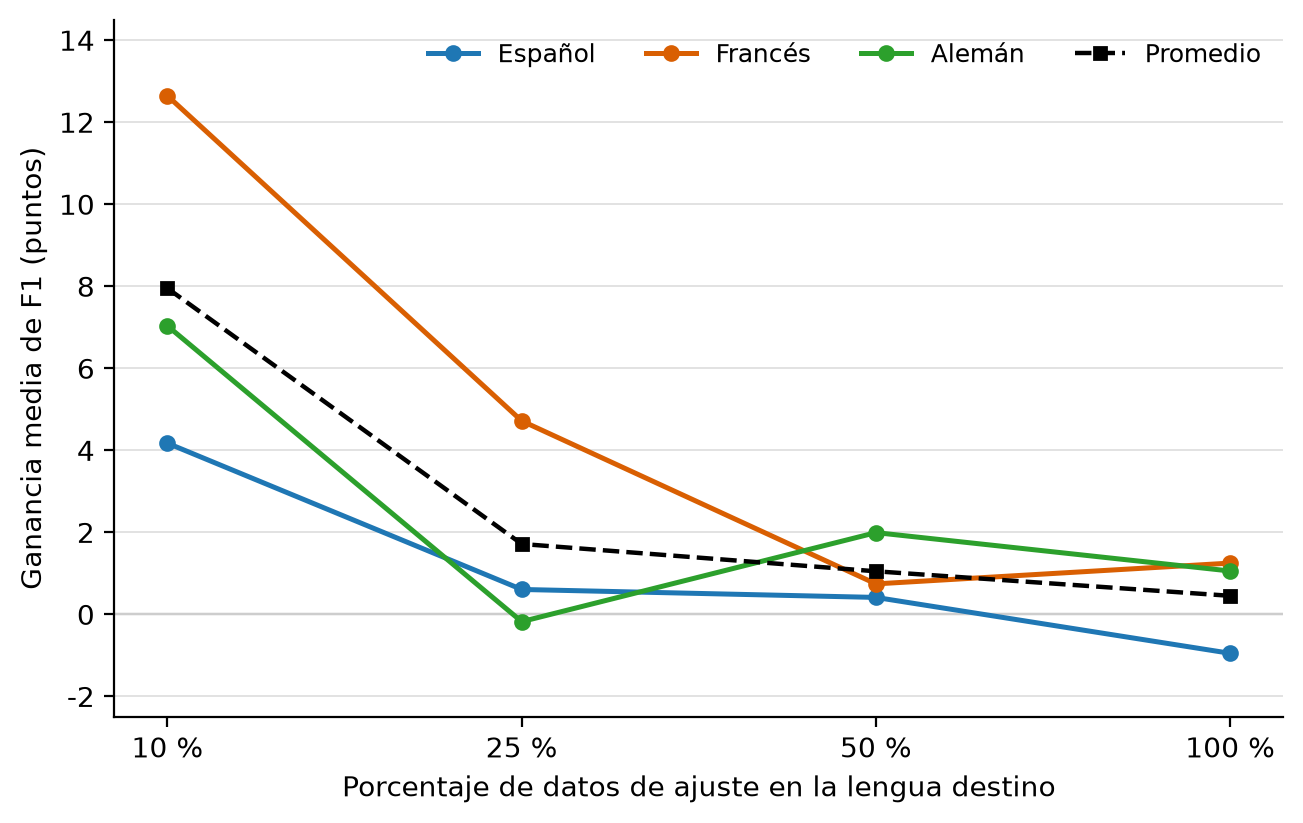
\includegraphics[width=0.78\textwidth]{figuras/ganancia_media.png}
\caption{Ganancia media en puntos de F1 por lengua y tamaño del conjunto de ajuste. Cada punto promedia los tres profesores ($B_p$, $B_{ft}$, $mB_{ft}$) frente a \textit{noKD}; la línea negra promedia las tres lenguas. Elaboración propia a partir de la Tabla~3 de \cite{piperno2025}.}
\label{fig:ganancia}
\end{figure}

El descenso de $+7{,}95$ a $+0{,}45$ tiene una explicación compatible con los datos: el baseline sube. Entre el 10\,\% y el 100\,\%, el noKD sube 16,78 puntos en español, 25,69 en francés y 22,96 en alemán. Cuanto más alto el punto de partida, menos espacio queda para la ganancia. Los autores añaden que la brecha entre BioBERT y mBERT sin destilación en inglés se reduce de unos 10 puntos con el 10\,\% a unos 5 con el 100\,\%. Con pocos datos el profesor aporta la frontera que las etiquetas no definen; con todos, el estudiante la aprende solo.

El ahorro de etiquetas es modesto. El mejor modelo destilado con el 10\,\% no alcanza al noKD con el 25\,\% en ninguna de las tres lenguas: 78,11 frente a 80,46 en español, 76,62 frente a 78,21 en francés y 73,30 frente a 78,34 en alemán. La destilación reduce las etiquetas necesarias, pero no sustituye 15 puntos porcentuales del corpus.

\subsection{Las cinco preguntas}

\textbf{Pregunta 1.} Sí se transfiere, con una precisión: «sin datos en inglés» significa sin etiquetas inglesas en el ajuste final. Con $B_p$, el delta es positivo en 11 de 12 configuraciones; la única excepción es $-0{,}03$ (español, 50\,\%). El conocimiento biomédico se transfiere, aunque el efecto dependa de la lengua y del tamaño de ajuste.

\textbf{Pregunta 2.} También se transfiere, aunque con más celdas negativas. $B_{ft}$ es positivo en 9 de 12 y $mB_{ft}$ en 8 de 12, con un cero. En el 100\,\%, $mB_{ft}$ pierde 1,77 en español y 1,49 en alemán.

\textbf{Pregunta 3.} Los autores no hallan diferencia clara entre $B_{ft}$ y $mB_{ft}$ y concluyen que el mBERT ajustado es más económico. $mB_{ft}$ gana 3 filas, $B_{ft}$ gana 3 y $B_p$ gana 6. Nuestra cautela es que $mB_{ft}$ comparte tokenizador y espacio de embeddings con el estudiante, así que parte de la ganancia podría deberse a esa cercanía.

\textbf{Pregunta 4.} La ganancia media cae de $+7{,}95$ a $+0{,}45$ entre el 10\,\% y el 100\,\%. La supervisión directa reemplaza la señal del profesor.

\textbf{Pregunta 5.} El RSA muestra una correlación de Pearson mayor entre profesor y estudiante después de la destilación, en las tres lenguas y con los tres profesores. Los estudiantes destilados se parecen más entre sí que al noKD. La correlación es más alta con $B_p$ que con los profesores ajustados; los autores lo atribuyen a que el ajuste especializa las capas finales. El RSA es una comprobación del mecanismo, no una prueba de comprensión clínica.

\subsection{MNRL frente a MSE}

MNRL supera a MSE en 32 de los 36 casos, con ventaja mayor cuando hay pocos datos. Los autores lo explican por la sensibilidad de MSE al ruido de la traducción. La comparación tiene dos límites: se reporta de forma gráfica y como conteo, sin tabla por celda, y el artículo presenta el brazo con MSE como reproducción de \cite{reimers2020}, pero la Figura~5 lo aplica a los mismos tres profesores. No se documenta qué se conservó de la receta original, así que la comparación es un cambio de pérdida sobre el flujo propio y no una reproducción verificable.

\section{Discusión crítica}
\label{sec:discusion}

El artículo \cite{piperno2025} plantea una pregunta pertinente y la responde con un diseño legible: un profesor entrenado en inglés, un estudiante multilingüe y una alineación de representaciones evaluada en tres lenguas y cuatro tamaños. La contribución es real en eficiencia de datos. Nuestra lectura es que la evidencia sostiene afirmaciones más estrechas que las que el texto formula.

\subsection{Validez interna}

Los autores no reportan semillas, repeticiones, desviaciones estándar, intervalos de confianza ni pruebas de significancia, y no consta que hayan hecho más de una corrida por configuración.

Con pruebas de 1.842 a 2.317 muestras, una diferencia de 0,1 puntos de F1 equivale a reclasificar un par de ejemplos si el F1 es micro; con macro, depende del tamaño de la clase. El $+0{,}11$ de $B_p$ en español con el 25\,\%, el $+0{,}30$ frente al $+0{,}17$ de $B_{ft}$ en alemán con el 25\,\% y el $+0{,}00$ de $mB_{ft}$ en francés con el 50\,\% caen en ese margen. La ventaja media que reportan los autores es de aproximadamente 0,70 puntos de $B_p$ sobre $B_{ft}$; la Tabla~3 da 0,78 al promediar las 12 diferencias, y ninguna de las dos tiene medida de dispersión. Los asteriscos convierten variación no medida en una decisión categórica. El resultado principal no depende de esas décimas: la caída de $+7{,}95$ a $+0{,}45$ puntos se repite en las tres lenguas y en los tres profesores.

La Tabla~\ref{tab:f1} reporta noKD absoluto y deltas, de modo que el lector debe sumar. Tampoco se define si el F1 es macro, micro o ponderado, y con 18 clases desbalanceadas la distinción pesa. La notación agrava la ambigüedad: el texto presenta los deltas con signo de porcentaje, mientras la tabla son puntos; leído como porcentaje relativo, $+12{,}89$ sobre 63,73 daría 8,21 puntos. Tres semillas y un bootstrap pareado cerrarían la brecha.

\subsection{Validez de constructo}

La Figura~3 describe el preprocesamiento como la creación de un conjunto «unbiased». El término designa la eliminación de muestras de prueba cuyo BLEU frente al entrenamiento traducido supera 0,3: un control de contaminación, no una auditoría de equidad. El filtro descansa en BLEU, que mide n-gramas, no significado: dos paráfrasis con el mismo contenido obtienen BLEU bajo y permanecen. El umbral 0,3 se justifica con una observación informal, sin muestra ni acuerdo interanotador. La calidad de la traducción no se mide: no hay COMET \cite{rei2020}, BERTScore \cite{zhang2020}, ida y vuelta ni revisión terminológica. La fidelidad de mBART en terminología médica queda sin evaluar.

Sin embargo, el filtro tampoco es neutro para la evaluación. Conserva entre el 40,8 y el 53,0\,\% de la prueba original, y el F1 se calcula, según la Tabla~2, sobre ese subconjunto. La Figura~2 del artículo muestra que la proporción por clase se mantiene, lo que atiende la composición pero no la dificultad. El sesgo de selección puede operar en ambas direcciones: si se eliminan duplicados fáciles, el F1 subestima el desempeño esperado; si se eliminan casos atípicos, lo sobreestima. La comparación interna es justa; lo que no se puede es leer ese F1 como desempeño en MSD.

El RSA se presenta como evidencia de transferencia. La pérdida empuja al estudiante hacia el profesor, así que una correlación mayor comprueba el mecanismo, no la comprensión clínica. Hay un confundidor: el profesor procesa inglés y el estudiante texto traducido, de modo que la correlación mezcla alineación con fidelidad de la traducción. Se calcula sobre millones de pares dependientes y se reporta sin intervalo.

La separación entre dominio y tarea se apoya en la identidad de los profesores, pero los tres combinan de forma distinta preentrenamiento y ajuste; el diseño no es factorial. «Sin datos en inglés» designa el escenario sin etiquetas inglesas en el ajuste, pero el inglés está presente en toda la destilación.

\subsection{Validez externa}

El corpus proviene de una sola fuente, MSD Manual Topics, con 18 macroclases. Los textos son educativos, no clínicos: no hay notas de historia clínica, laboratorio, transcripciones ni literatura primaria. La tarea es clasificación temática, no extracción de entidades ni codificación diagnóstica. Las tres lenguas son de altos recursos; «low-resource» describe el régimen de datos, no la lengua. El español se trata como un bloque único, sin variedades ni textos colombianos.

El artículo compara contra noKD, contra MSE y contra las curvas de BioBERT y mBERT de la Figura~4, pero faltan baselines. Falta translate-train: ajustar mBERT sobre el texto traducido con etiquetas inglesas y sin destilación, que separaría el valor de los datos traducidos del valor de la alineación. Faltan TF-IDF con un clasificador lineal, que en 18 clases y unas 12.000 muestras es un competidor serio, y BETO \cite{canete2020} o MarIA \cite{gutierrez2022}. Sin ellos no se sabe si mBERT era el estudiante adecuado.

\subsection{Reproducibilidad y transparencia}

El artículo no declara disponibilidad de código. Faltan el tamaño de lote, que en MNRL define los negativos; el valor de $\alpha$; la tasa de aprendizaje, épocas y criterio de parada; el pooling; y el peso de las dos alineaciones. La receta del baseline tampoco se detalla: para que el delta mida destilación y no presupuesto de ajuste, noKD y los estudiantes deberían compartir hiperparámetros. La comparación con MSE es una reimplementación sin detalle de fidelidad. El RSA usa $N = 4.300$ mientras la Tabla~2 reporta 4.295; no cambia conclusiones, pero es un artefacto. mBART-large-50 es de 2020 y no se compara con otros traductores.

\subsection{Ética y despliegue}

No hay evaluación de sesgo: ni WEAT, ni StereoSet \cite{nadeem2021}, ni CrowS-Pairs \cite{nangia2020}, ni métricas desagregadas. La destilación puede transportar estereotipos del corpus inglés a las tres lenguas. La etiqueta «unbiased» agrava el riesgo. No hay validación clínica: ni adjudicación por médicos, ni análisis de errores por gravedad. La motivación de acceso equitativo es más amplia que la evidencia. El análisis de privacidad está ausente; el corpus es público, pero el despliegue implicaría datos de pacientes.

La evidencia sostiene que la alineación mejora la eficiencia de datos en clasificación temática multilingüe sobre un corpus divulgativo. No sostiene que el estudiante comprenda el dominio clínico, que el resultado sea equitativo ni que sea desplegable en atención en salud.

\section{Conexión con los conceptos del curso}
\label{sec:curso}

El artículo \cite{piperno2025} se deja leer como una cadena de decisiones que el curso trata por separado. Cada etapa del flujo de procesamiento activa un concepto distinto y la correspondencia ayuda a ver por qué el método funciona y dónde pierde sustento.

Las representaciones contextuales son el sustrato. BERT produce un vector distinto para cada aparición de una palabra, y mBERT comparte un vocabulario de subpalabras entre lenguas, lo que permite que el mismo encoder procese español, francés y alemán \cite{devlin2019}. BioBERT conserva la arquitectura y desplaza la geometría hacia el vocabulario biomédico \cite{lee2020}. Que profesor y estudiante pertenezcan a la misma familia es una condición del diseño, porque una pérdida de distancia entre embeddings exige espacios comparables. El artículo usa [CLS] en el RSA, una decisión discutible: [CLS] se entrena para la predicción de la oración siguiente, no para similitud, y Sentence-BERT suele usar la media \cite{reimers2019}. El texto no especifica el pooling de la destilación.

La transferencia y la adaptación de dominio explican la jerarquía de profesores. mBERT representa el preentrenamiento general, BioBERT la adaptación al dominio y los modelos ajustados la adaptación a la tarea. La curva del 10 al 100\,\% es un experimento de eficiencia de datos. Una alternativa que el artículo no prueba es continuar el preentrenamiento de mBERT con texto biomédico en español antes de destilar: atacaría el problema desde el estudiante y permitiría comparar qué rinde más.

La destilación de características da nombre al método. El estudiante imita representaciones, no logits; la cabeza de clasificación del profesor no se transfiere. Eso explica por qué el estudiante puede ajustarse después con etiquetas en la lengua meta. También explica el alcance de la evidencia: el RSA verifica que la geometría se acercó, no que el contenido clínico se conservó. Una alternativa sería destilar sobre los 18 logits del profesor o combinar ambas señales.

El aprendizaje contrastivo aclara la pérdida. MNRL es la entropía cruzada de una softmax sobre similitudes: el positivo es la contraparte y los negativos son los demás pares del lote. El tamaño de lote define la dificultad y $\alpha$ cumple un papel parecido a la temperatura. MSE obliga a igualar coordenadas; la pérdida contrastiva solo exige que el positivo quede por delante. Una alternativa sería el minado de negativos difíciles o una pérdida contrastiva supervisada con las 18 clases.

La clasificación y el F1 cierran el ciclo. El ajuste final es una clasificación de 18 clases, y el F1 es el resumen. Macro, micro y ponderado responden preguntas distintas: macro promedia las clases por igual, micro acumula aciertos y ponderado pesa por soporte. Sin esa definición, el número de la Tabla~\ref{tab:f1} no se puede interpretar. Las matrices de confusión ofrecen la vista por clase que el promedio oculta, y el artículo las usa para comparar estudiantes, no para analizar errores. Una alternativa sería reportar F1 macro con soporte por clase y un bootstrap pareado.

Un enfoque lingüístico o de reglas sobre léxico terminológico, con la CIE-10 o el CUPS, sería más interpretable y auditable, pero más frágil ante variación, abreviaturas y texto libre. El artículo no lo compara; su ausencia confirma que la comparación es entre variantes de aprendizaje profundo, no entre familias de métodos.

\section{Preguntas del foro}
\label{sec:foro}

Las dos preguntas finales tienen naturalezas distintas. La primera es de ingeniería: cuándo el costo de traducir y destilar se paga con la mejora. La segunda es de validez: qué evidencia haría falta para llevar el resultado a textos clínicos colombianos. Una respuesta afirmativa a la primera no dice nada sobre la segunda.

\subsection{¿Cuándo justifica la mejora añadir traducción y destilación al entrenamiento?}

La ganancia reportada \cite{piperno2025} depende del déficit de etiquetas: el aumento medio es de 7,95 puntos de F1 con el 10\,\% de los datos, 1,72 con el 25\,\%, 1,05 con el 50\,\% y 0,45 con el 100\,\%. El máximo es de 12,89 puntos en francés con el 10\,\% y el profesor $mB_{ft}$; el mínimo, de $-1{,}77$ en español con el 100\,\% y ese mismo profesor. Siete de las 36 celdas son negativas.

El primer criterio combina la escasez de etiquetas y la calidad del profesor. Con el 10 o el 25\,\% del corpus, la mejora esperada supera los 1,7 puntos en promedio y llega a dos dígitos en algunas combinaciones; con el corpus completo cae por debajo de medio punto y aparecen pérdidas. El BioBERT preentrenado supera en promedio al ajustado en aproximadamente 0,70 puntos, según los autores; la Tabla~3 da 0,78 al promediar las 12 diferencias. No hace falta anotar en inglés para tener profesor. La lectura por celda matiza: con el 100\,\% de los datos, el ajustado supera al preentrenado por 0,30 en alemán y cae 1,71 puntos por debajo del baseline en español. La elección debería validarse con el corpus destino.

El segundo criterio combina la calidad de la traducción y la comparación con translate-train. mBART es general y el artículo no usa léxico especializado, ida y vuelta, COMET ni BERTScore. MNRL rinde mejor que el error cuadrático medio en 32 de 36 casos; los autores lo atribuyen a la sensibilidad de MSE al ruido. Pero tolerar no es corregir: un par que invierte una negación se aprende junto con el conocimiento. Donde el término tiene consecuencia, hace falta control terminológico antes de entrenar. El artículo contrasta contra el ajuste directo y contra el error cuadrático medio, no contra entrenar con traducciones sin destilar, ni contra TF-IDF, ni contra BETO o MarIA. Sin esa comparación, la mejora incluye el efecto de aumentar los datos. Si un clasificador simple sobre traducciones empata, no se justifica mantener dos alineaciones, un traductor y un profesor.

El tercer criterio combina el costo y la significancia. La destilación no reduce el costo de inferencia: el estudiante es mBERT, del mismo tamaño que el baseline, así que en producción se ejecuta el mismo modelo. Lo que se reduce es la anotación. Traducir el conjunto inglés de 11.860 muestras a las tres lenguas y ejecutar la alineación añaden cómputo de entrenamiento, no de despliegue. No se reportan semillas ni repeticiones ni intervalos, y no consta que haya más de una corrida por configuración. Varias diferencias son de 0,11, 0,17, $-0{,}03$ y $-0{,}04$ puntos, inseparables del ruido. Solo un delta sostenido en varias semillas, con un intervalo que excluya el cero, justifica cambiar la arquitectura; mientras no exista, una diferencia menor a un punto es un empate.

El cuarto criterio es el riesgo clínico. El filtro de similitud por BLEU conservó entre el 40,8 y el 53,0\,\% de la prueba original, y las cifras se calculan sobre esa parte. Una mejora que dependa de la selección no se sostiene en una distribución sin filtrar.

Añadiríamos traducción y destilación con hasta el 25\,\% de las etiquetas, sin modelo local disponible, terminología verificada, ventaja medida sobre translate-train y un delta que sobreviva a la variación entre semillas. Si falla la terminología, si el baseline empata o si no hay repeticiones, conviene anotar más datos.

\subsection{¿Qué evidencia exigiríamos para transferir este resultado a textos médicos de Colombia?}

El corpus son manuales MSD en cuatro lenguas, con traducciones automáticas del inglés para la destilación. El texto clínico colombiano es otra cosa: notas de evolución, epicrisis, laboratorio, triage y facturación. Cambian el vocabulario, la longitud, la sintaxis, las abreviaturas y la variedad del español. La transferencia exige una escalera de evidencia.

El primer escalón es la reproducción. No se precisa si el F1 es macro, micro o ponderado, y con 18 clases desbalanceadas eso cambia el número; tampoco se declara código ni se reportan semillas. Pediríamos reejecución con la partición original, varias semillas y la agregación declarada.

El segundo es la validación externa con textos clínicos locales. Antes de entrenar se mide el cambio de distribución: vocabulario, longitud y proporción de términos fuera del vocabulario de mBERT frente al corpus de origen. Si esa proporción es alta, la caída es esperable y debe cuantificarse.

El tercero es la taxonomía y la anotación. Las 18 clases no equivalen a la CIE-10, al CUPS ni a los grupos de la RIAS; el mapeo directo pierde granularidad y algunas categorías mezclan tema y audiencia. Hay que decidir si se conserva la taxonomía del manual o se construye una propia. La anotación debe hacerla al menos dos clínicos, con kappa de Cohen o de Fleiss por clase y adjudicación. Si el desacuerdo entre expertos supera el delta que se quiere detectar, el experimento no resuelve la pregunta.

El cuarto son los baselines y la robustez. BETO \cite{canete2020} y MarIA \cite{gutierrez2022} ajustados con datos colombianos, y TF-IDF con regresión logística. Si un encoder en español con datos locales iguala al estudiante destilado, la premisa del artículo deja de aplicarse. Hay que probar abreviaturas, errores de digitación, siglas institucionales y nombres comerciales. La tolerancia de MNRL se midió contra ruido de traducción, no contra ruido de escritura clínica.

El quinto es la calibración y la equidad. Un clasificador que orienta derivaciones necesita probabilidades calibradas: error de calibración esperado y curvas de fiabilidad por clase. Exigiríamos métricas desagregadas por región, género, régimen de afiliación y edad; diez puntos de diferencia entre contributivo y subsidiado invalidarían el uso aunque el promedio fuera alto.

El sexto es el cumplimiento y la reproducibilidad. La Ley 1581 de 2012 trata los datos de salud como sensibles y exige autorización y finalidad; la Resolución 1995 de 1999 regula la historia clínica y su reserva. Añadiríamos aval de comité de ética y anonimización verificable. La reproducibilidad exige código, semillas, checkpoints, ficha de modelo y lectura de errores por clínicos. La pregunta que decide el despliegue es si los errores son tolerables en el uso previsto, no cuántos puntos sube el F1.

La evidencia que consideraríamos insuficiente es fácil de enumerar: una mejora sobre la prueba de MSD, que no representa el texto colombiano; un BLEU alto, que mide solapamiento léxico; una correlación alta en el análisis de representaciones, que solo confirma la alineación; una corrida única con dos puntos de diferencia; una demostración con veinte ejemplos; un benchmark sin datos locales. En Colombia no faltan manuales traducidos, faltan corpus clínicos anotados y gobernados. La evidencia que pediríamos separa una mejora de benchmark de un instrumento clínico.

\section{Preguntas de clase}
\label{sec:clase}

Las tres preguntas comparten un supuesto: la calidad de un modelo multilingüe no se agota en su F1. Las respondemos en el orden en que surgieron.

\subsection{¿Puede la destilación transferir sesgos de género y estereotipos a otras lenguas?}

Es posible en principio, y el mecanismo es geométrico. La destilación de características que evalúa \cite{piperno2025} no copia etiquetas: alinea la geometría del estudiante con la del profesor, de modo que las distancias relativas entre representaciones pasan a ser el objetivo de aprendizaje. El sesgo vive en esa geometría, no en las etiquetas. Caliskan et al.\ \cite{caliskan2017} mostraron que los embeddings absorben asociaciones humanas presentes en el corpus, y ese es el material que MNRL empuja a reproducir. Si en el espacio del profesor las oraciones sobre enfermería están más cerca de las de mujeres que de las de hombres, o si cierta enfermedad aparece asociada a un grupo, esa relación forma parte de la estructura que la pérdida aproxima. El estudiante puede aprenderla sin ver una etiqueta de género. Nadeem et al.\ \cite{nadeem2021} y Nangia et al.\ \cite{nangia2020} documentan asociaciones estereotipadas en modelos preentrenados, y la destilación es una vía para que viajen de una lengua a otra.

El español, el francés y el alemán añaden el género gramatical. El inglés \textit{the patient} no marca género; la traducción debe elegir entre \textit{el paciente} y \textit{la paciente}, entre \textit{der Patient} y \textit{die Patientin}. mBART \cite{liu2020} decide con los datos paralelos con los que fue entrenado y puede introducir sus propios estereotipos. El par que recibe el estudiante carga un género que el original no codificaba, y la alineación lo trata como parte del significado. El género impuesto por la traducción puede amplificar la asociación que el profesor ya tenía. En todo el flujo no hay un paso que retire esa asociación.

La formulación defendible es que el estudiante puede heredar y, en algunos casos, amplificar. La destilación es una proyección con pérdida: el estudiante tiene otro tokenizador y otra capacidad; el ajuste posterior puede atenuar o reforzar la asociación; y el ruido de traducción no es sesgo del profesor. Con los datos publicados no se puede afirmar la reproducción exacta ni descartarla.

Lo que el artículo no hace es medir el sesgo. No hay WEAT ni SEAT, no hay StereoSet ni CrowS-Pairs, y no hay métricas desagregadas por género. El término \textit{unbiased} de la Figura~3 se refiere a la dissimilaridad medida con BLEU entre la prueba y el entrenamiento traducido, no a equidad.

\subsection{¿Qué estrategias permiten reducir esos sesgos?}

La primera es medir. Antes de elegir un método hay que establecer una línea base de sesgo en las representaciones del estudiante, antes y después de la destilación, con SEAT sobre las representaciones de oración, con pares contrafactuales que cambien solo el género o el origen y con métricas desagregadas por grupo. Sin esa medición no hay forma de saber si una intervención funcionó.

La segunda es intervenir sobre los datos: aumentar ejemplos contrafactuales, equilibrar plantillas y traducir las dos variantes de una frase para que el traductor no elija una sola. En un corpus de manuales médicos, esto significa incluir descripciones de pacientes y profesionales en ambas formas y revisar que ginecología no quede asociada automáticamente con un género.

La tercera es intervenir sobre las representaciones. INLP \cite{ravfogel2020} proyecta iterativamente sobre el espacio nulo de clasificadores lineales del atributo; SentenceDebias \cite{liang2020} resta una dirección de sesgo estimada en embeddings de oración. Ambos exigen declarar el atributo que se quiere retirar y tienen un costo: es esperable que \textit{Gynecology and obstetrics} y \textit{Women's health issues} correlacionen con el género (el artículo no lo mide), de modo que eliminar la dirección puede borrar señal útil. El compromiso entre equidad y exactitud debe medirse.

La cuarta es calibrar por grupo y evaluar con hablantes nativos y clínicos, porque un estereotipo en español sobre \textit{la enfermera} no coincide con el del inglés ni con el de una región colombiana. La quinta es documentar: fichas de modelo, auditoría de los datos de traducción y reporte de métricas por grupo antes de cualquier despliegue.

BLEU y MNRL no son mecanismos antisesgo. BLEU mide solapamiento de n-gramas y MNRL es una pérdida de ranking; ninguna tiene noción de atributo protegido. El filtro de BLEU retira muestras de prueba semejantes al entrenamiento y cambia la distribución, no la equidad. Ningún método elimina el sesgo por completo; el objetivo es acotarlo, medirlo y documentarlo con un umbral de tolerancia declarado.

\subsection{¿Cómo se garantiza la equivalencia semántica?}

MNRL garantiza un orden relativo dentro del lote, no equivalencia de significado. La pérdida exige que el par positivo esté más cerca que los negativos del lote, y nada en ella afirma que la traducción sea correcta. Si el par es falso, el modelo aprende a acercar un par falso. La composición del lote determina qué contrastes se aprenden, y el artículo no describe cómo muestrea los negativos ni reporta el tamaño de lote o el valor de $\alpha$.

BLEU es léxico: compara n-gramas con una referencia y es insensible a una negación invertida, a un cambio de dosis o a un error de lateralidad. «No presenta dolor» y «presenta dolor» comparten casi todos sus n-gramas. mBART, además, puede mistraducir términos médicos, y el artículo no emplea léxico especializado, ida y vuelta, COMET \cite{rei2020} ni BERTScore \cite{zhang2020}. El umbral de 0,3 se aplica para filtrar la prueba, no para validar los pares.

mBERT \cite{devlin2019} es generalista, entrenado sobre Wikipedia en 104 lenguas, y su cobertura del español clínico es, en principio, limitada; el artículo no la mide. Sin embargo, el artículo ya prueba el conocimiento de dominio en las preguntas 1 y 3: compara BioBERT preentrenado, BioBERT ajustado y mBERT ajustado como profesores. El profesor preentrenado supera en aproximadamente 0,70 puntos en promedio al ajustado, según los autores, y un profesor generalista produce mejoras comparables. La limitación no es que nadie haya comprobado el dominio; la comprobación existe y su resultado es que la ventaja es pequeña. Un estudiante BETO \cite{canete2020} o MarIA \cite{gutierrez2022} tendría mejor cobertura del español, pero trasladaría el problema: la equivalencia y el sesgo seguirían sin medirse.

Un preentrenamiento continuo con corpus médicos multilingües mejoraría la cobertura de dominio, pero no garantiza la equivalencia: un modelo puede mejorar en español médico y aun así invertir una negación. Tampoco eliminaría la validación humana; cambiaría qué debe revisar.

Nuestra propuesta combina controles en la traducción y en la evaluación: léxico especializado y restricciones terminológicas de la CIE-10, el CUPS y nombres de medicamentos; ida y vuelta con comparación; COMET y BERTScore como medidas complementarias, con sus límites; negativos duros que difieran solo en negación, temporalidad, dosis o lateralidad; y anotación experta de una muestra estratificada. La calidad de los pares debería evaluarse por separado del F1, algo que el artículo nunca hace. La equivalencia es una propiedad empírica de cada par y se audita; no se deduce de la pérdida.

\section{Reflexión del equipo}
\label{sec:reflexion}

La lectura del artículo nos dejó tres aprendizajes. El primero es que la destilación de conocimiento es una técnica de eficiencia de datos, no una técnica de equidad. El artículo la presenta dentro de un marco de inclusión lingüística, pero su experimento mide exactitud temática en tres lenguas europeas. Confundir el marco con la medición lleva a atribuirle propiedades que el diseño no prueba.

El segundo es que la evidencia es más estrecha que la cifra principal. La ganancia de 12,89 puntos existe, pero corresponde a una celda: francés, 10\,\% de los datos y profesor $mB_{ft}$. El promedio cae de 7,95 a 0,45 puntos cuando se pasa del 10 al 100\,\%, y siete de las 36 celdas son negativas. Un lector que solo retenga el máximo se queda con la parte más favorable de una distribución heterogénea.

El tercero es que las métricas son aproximaciones. El F1 mide aciertos sobre una prueba filtrada; BLEU mide solapamiento léxico; la correlación de RSA mide cercanía geométrica. Ninguna de las tres mide comprensión clínica, equidad o equivalencia semántica. Cada una acota un tipo de afirmación y ninguna cubre las demás.

La discusión de clase confirmó que el sesgo viaja por la geometría, que mitigarlo exige medir y auditar, y que la equivalencia semántica se audita par a par.

Nuestro análisis tiene límites. No replicamos los experimentos, no tuvimos acceso al código ni a las traducciones, y no anotamos textos colombianos. Trabajamos sobre las cifras reportadas y sobre el texto del artículo. Por eso hablamos de lo que la evidencia permite sostener, no de lo que ocurriría si repitiéramos el entrenamiento.

Quedan preguntas abiertas. ¿Cómo se construiría un benchmark biomédico colombiano con anotación clínica y gobernanza de datos? ¿Qué método de mitigación de sesgo resiste la evaluación en español médico sin borrar señal útil? ¿Un estudiante BETO o MarIA superaría a mBERT en este corpus? ¿Cuánto cuesta un error de traducción en una decisión clínica y cómo se detecta antes del despliegue? El artículo no las responde; su aporte es haber abierto un camino viable para plantearlas.

\section{Conclusiones}
\label{sec:conclusiones}

El artículo \cite{piperno2025} muestra que la destilación de conocimiento con Sentence Transformers puede transferir conocimiento biomédico desde el inglés hacia el español, el francés y el alemán cuando hay pocas etiquetas. La ganancia media cae de 7,95 puntos de F1 con el 10\,\% de los datos a 0,45 con el 100\,\%, y la dirección del efecto se repite en las tres lenguas y en los tres profesores. El máximo de 12,89 puntos corresponde a una sola celda y no debe leerse como el resultado típico.

Sin embargo, la contribución es real en eficiencia de datos, no en equidad ni en validez clínica. El artículo no mide sesgo, no valida la calidad de las traducciones y no evalúa texto clínico. Su corpus son manuales educativos, sus lenguas son de altos recursos y su prueba está filtrada por similitud con el entrenamiento traducido. Esas condiciones acotan lo que puede concluirse: el método funciona en clasificación temática sobre prosa divulgativa, con un profesor inglés y un estudiante multilingüe, en el régimen de pocos datos.

Las cinco preguntas reciben respuestas convergentes. Añadir traducción y destilación se justifica con hasta el 25\,\% de las etiquetas, un profesor con conocimiento de dominio o de tarea, terminología verificada y una ventaja que supere a translate-train y a la variación entre semillas. Transferir el resultado a Colombia exige validación externa, taxonomía local, anotación clínica, baselines BETO, MarIA y TF-IDF, calibración, equidad y cumplimiento normativo. La destilación puede transferir y amplificar sesgos; reducirlos exige medirlos, intervenir datos y representaciones y auditar. La equivalencia semántica no se garantiza con MNRL ni con BLEU: se audita con léxico especializado, ida y vuelta, métricas semánticas y anotación experta.

El balance final es favorable al artículo como método y cauteloso como evidencia. Aporta un diseño replicable y una pregunta pertinente; deja abiertos la varianza, la definición de la métrica, la calidad de la traducción, el sesgo y la validación local. La destilación multilingüe merece probarse en Colombia, pero solo después de construir el corpus, la taxonomía y la evaluación que permitan saber si funciona.


\nocite{*}
\bibliographystyle{apalike}
\bibliography{references}

\end{document}
